% !TEX root = ../main.tex

\section{Implementácia ovládača}
\label{sec:program}

\begin{figure}[!htbp]
	\begin{center}
		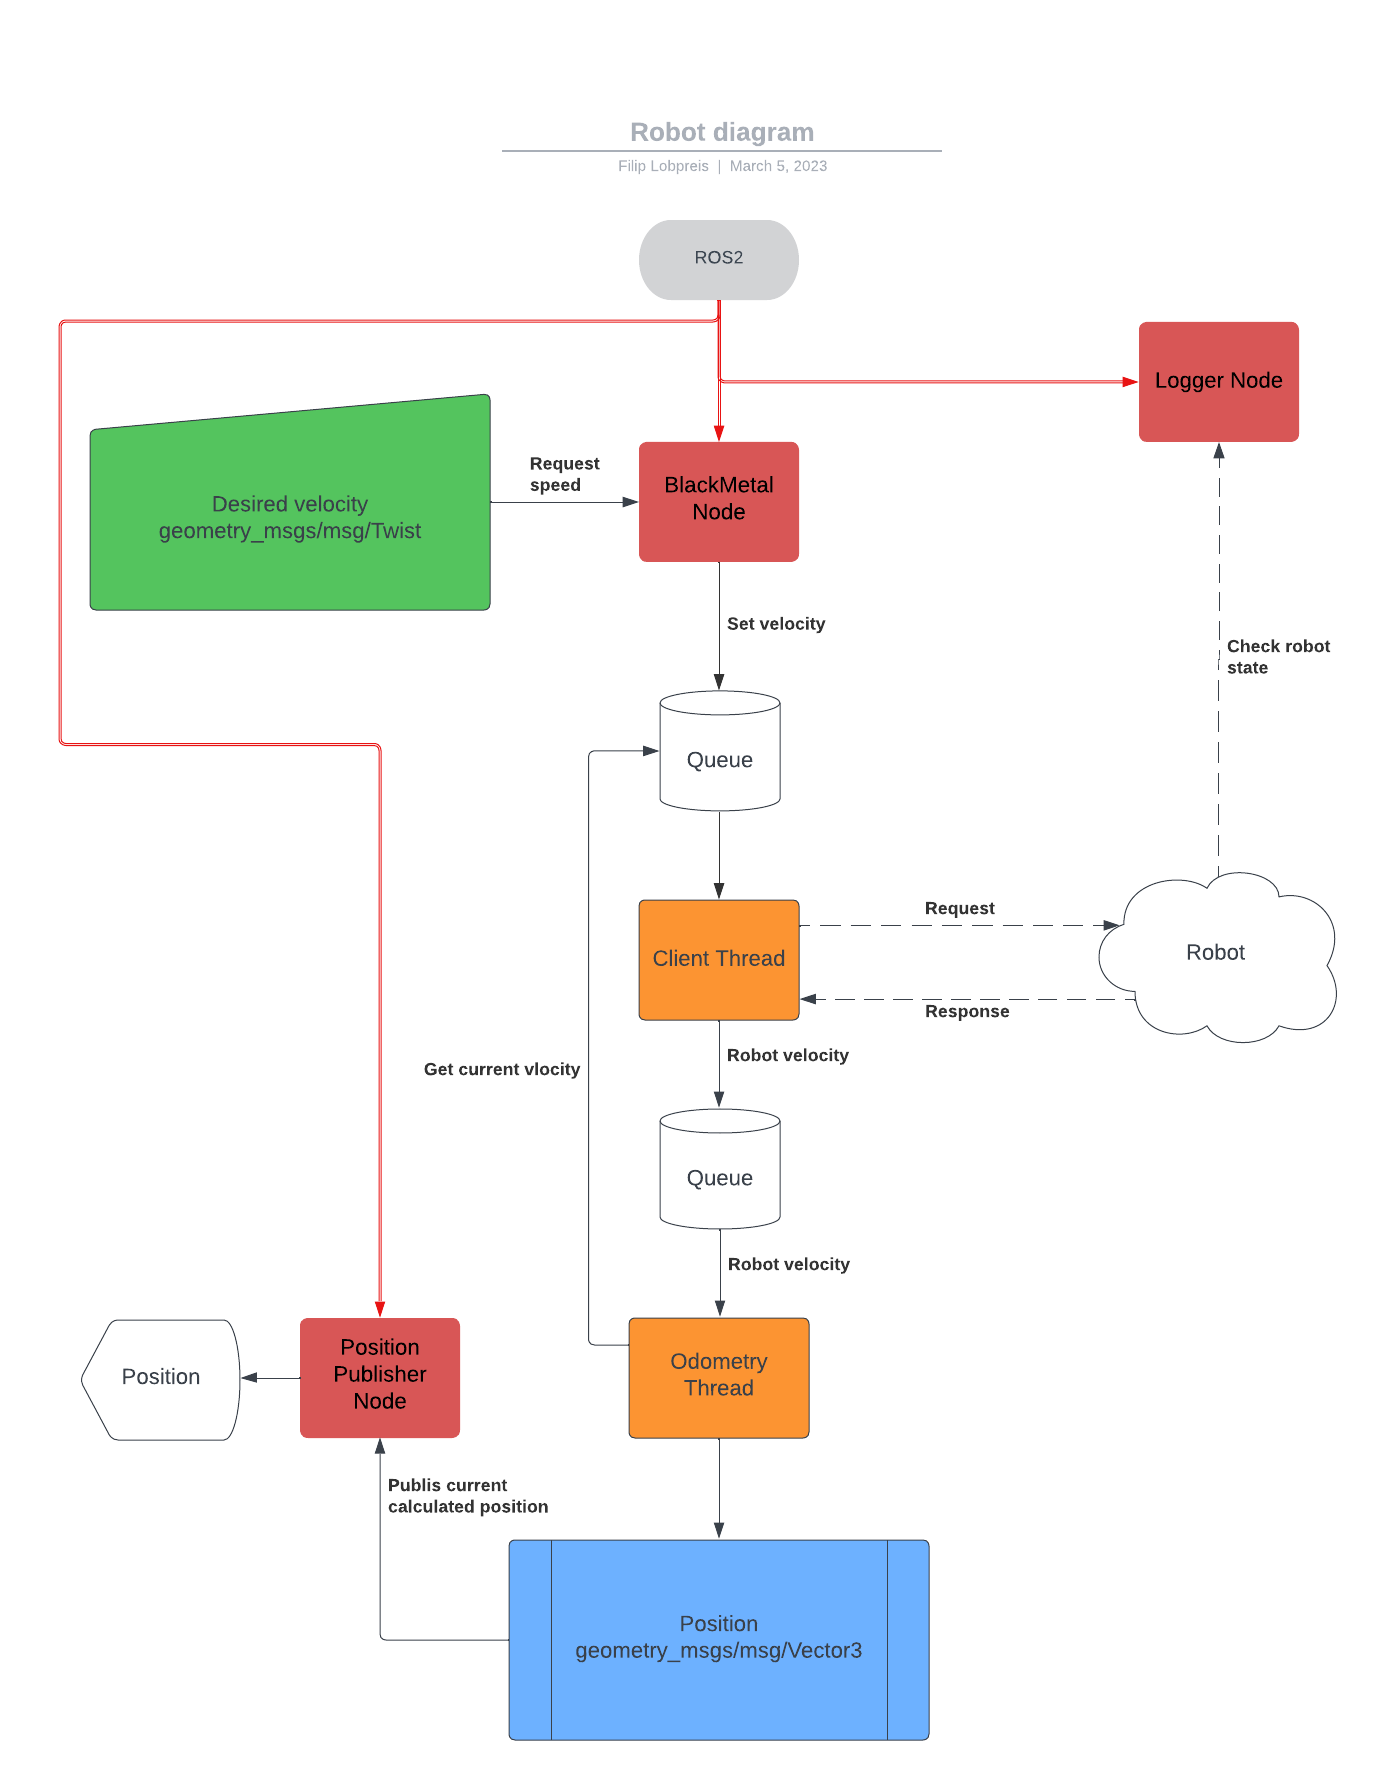
\includegraphics[width=0.9\textwidth]{img/BlackMetal_flowchart.png}
	\end{center}
	\caption{Graf vykonávania programu na~ovládanie robota pomocou ROS2.}
	\label{fig:flowchart}
\end{figure}

Cieľom kapitoly je navrhnúť a~implementoval ovládač v~prostredí ROS2, ktorý komunikuje s~robotom
cez~protokol TCP/IP. Na~obrázku Obr.~\ref{fig:flowchart} môžeme vidieť viacero objektov rôznych
farieb. Objekty zobrazené červenou farbou sú~uzly spracovávané a~vytvárané v~rámci ROS2. Každý
tento objekt sa vykonáva v~osobitnom procese. Objekty zobrazené oranžovou farbou sú~objekty, ktoré
majú svoje vlastné vlákno. Tieto objekty boli vytvorené uzlom BlackMetal. Dátové štruktúry Queue,
zobrazené bielou farbou sú~vytvorené tak, aby zabezpečovali bezchybnú komunikáciu a~synchronizáciu
medzi viacerými vláknami. Objekt so~zelenou farbou je vstup do~programu. Je zadávaný užívateľom
a~reprezentuje žiadanú rýchlosť robota. Modrý objekt je výstupom programu. Je to~téma, na~ktorú
sa publikuje aktuálna pozícia robota. Robot samotný je zobrazený bielou farbou vo~forme malého
obláčika. Prerušované čiary na~diagrame znázorňujú sieťovú komunikáciu ovládača a~robota. Červené
dvojité čiary udávajú, ktoré objekty patria ROS-u. Nakoniec čierne plné čiary reprezentujú tok dát
medzi objektmi.

\subsection{Uzly}
\label{subsec:nodes}

Na~obrázku Obr.~\ref{fig:flowchart} môžeme vidieť postup vykonávania programu na~ovládanie
robota BlackMetal pomocou ROS2. Na~začiatku programu sa vytvoria 3 uzly.

\begin{itemize}
	\item \textbf{Position Publisher} -- uzol, na~ktorý sa publikuje vypočítaná pozícia robota.
		Tento uzol existuje v~programe len na~overenie publikovaných informácii a~ich následné uchovávanie,
	\item \textbf{Logger} -- uzol slúžiaci na~zaznamenávanie stavu robota~\ref{sec:logovanie},
	\item \textbf{BlackMetal} --  uzol ovládajúci robot podľa zadaných dát užívateľom.
\end{itemize}

\subsection{Vstup}
\label{subsec:input}

Uzol \textbf{BlackMetal} vytvorí príjemcu, ktorý počúva na~téme \textbf{/cmd\_vel} a~príma správy typu
\textit{geometry\_msgs/msg/Twist}. Tento vstup je vo~forme príkazu zadaného v~príkazovom riadku. Vyzerá nasledovne:

\lstset{language=bash,
	basicstyle=\ttfamily,
	keywordstyle=\color{blue}\ttfamily,
	stringstyle=\color{orange}\ttfamily,
	commentstyle=\color{green}\ttfamily,
	morecomment=[l][\color{magenta}]{\#},
	numberstyle=\color{red}
}

\label{requestCommand}
\begin{lstlisting}[language=bash]
	ros2 topic pub /cmd_vel geometry_msgs/msg/Twist
		"linear:
			x: 0.0,
			y: 0.0,
			z: 0.0,
		angular:
			x: 0.0,
			y: 0.0,
			z: 0.0" -1
\end{lstlisting}

Tento \hyperref[requestCommand]{príkaz} publikuje jednu správu (\textit{-1}) na~tému \textit{/cmd\_vel}.
Obsahuje lineárne a~uhlové rýchlosti. Z~tejto správy sa využijú dva údaje lineárna rýchlosť
po~osi \textit{x} a~uhlová rýchlosť po~osi \textit{z}. Ostatné lineárne rýchlosti neovplyvňujú
chod robota rovnako ako ďalšie uhlové rýchlosti. Táto správa typu \textit{geometry\_msgs/mgs/Twist}
je následne spracovaná a~uložená do~rady \textit{Queue}. Táto rada je prioritne založená.
To~znamená, že~požiadavka s~nižším kódom ma vyššiu prioritu. Požiadavky a~ich kódy môžeme vidieť v~sekciách \ref{sec:ovladanie} a~\ref{subsec:extendRobotCommands}.

\subsection{Komunikácia s~robotom}
\label{sec:robotComms}

Ako je naznačené na~Obr.~\ref{fig:flowchart}, klient si vo~svojom vlastnom vlákne vytiahne
prvú správu z~rady a~pretransformuje ju do~formy JSON. Tento typ správy môžeme vidieť v~sekcii
\ref{sec:ovladanie}. Príkaz je poslaný robotu a~ten obratom dá vedieť, či~danú požiadavku obdržal.
Ak~obsah tejto správy žiadal o~vrátenie rýchlostí kolies, tak~robot ďalšou správou odpovie
na~danú požiadavku. Typ tejto odpovede môžeme vidieť v~\ref{jsonWannabeSpeed}. V~tomto prípade
sa správa spracuje a~uloží sa do~ďalšej rady.

\subsection{Odometria}
\label{sec:odometria}

Odometria, počítanie polohy na~základe rýchlostí kolies, sa vykonáva rovnako ako komunikácia
s~robotom, v~separátnom vlákne. Tu je potreba si uvedomiť jednu skutočnosť. To~je tá, že~keď
posielame žiadosť na~nastavenie rýchlostí kolies robota, tak~robot si hodnoty v~žiadosti prepočíta.
Prepočítané dáta následne poskytne enkóderom. Keď si ale~tieto rýchlosti vyžiadame z~enkóderov,
tak~sa robot týchto dát nechytá a~my si ich musíme prepočítať na~metre za~sekundu. Aby sme dostali
rýchlosti kolies od~robota, tak~si ich musíme od~neho vypýtať. Ako sme už~spomenuli v~kapitole~\ref{sec:robotComms},
tieto správy majú nižšiu prioritu ako nastavenie rýchlosti kolies alebo bezpečnostné zastavenie
robota. Preto~sa môže stať, že~správy posielané robotu nebudú dodržiavať presne stanovenú frekvenciu
v~čase keď mu bude užívateľ posielať príkazy. Toto nám až tak~neprekáža, lebo server na~robote sme upravili, tak aby tieto
spravy prijímal neustále (kapitola~\ref{subsec:communicationDelay}).

Po~obdržaní rýchlostí robota v~impulzoch za~sekundu si tieto dáta kvôli zašumeniu preženieme cez~filter
a~následne ich spracujeme. Spracovanie prebieha nasledovne:

\begin{enumerate}
	\item Prepočítanie rýchlostí kolies robota z~impulzov za~sekundu na~metre za~sekundu,
	\item Prepočítanie lineárnej a~uhlovej rýchlosti robota na~jeho ťažisko,
	\item Zistenie aktuálnej zmeny času oproti predchádzajúcemu meraniu,
	\item Zapísanie aktuálneho času, lineárnej a~uhlovej rýchlosti do~spravy,
	\item Prepočítanie aktuálnej polohy z~nameraných rýchlostí.
\end{enumerate}

Za~cieľom počítania odometrie sme si odmerali polomer kolies a~vzdialenosť stredov týchto kolies.
\textit{Polomer kolies} (\textbf{R}) sme určili na~\textbf{0,08m}. \textit{Polomer stredov kolies}
\textbf{L} robota sme určili na~\textbf{0,56m}. Z~dokumentácie robota \cite{encoder} sme si zistili
\textit{rozsah enkóderov} (\textbf{E}) (\textbf{1024} impulzov na~otočku)  Tieto údaje sme použili
na~prepočítanie impulzov za~sekundu na~metre za~sekundu.

\begin{equation}
	V_{mps} = \frac{2 \pi R}{E} v_{imp}
	\label{eq:vmps}
\end{equation}

Týmto spôsobom si vieme prepočítať rýchlosti pre~pravé a~ľavé koleso robota.
V~druhom bode sme si prepočítali lineárnu a~uhlovú rýchlosť pomocou rýchlosti pravého a~ľavého kolesa.

\begin{equation}
	V_{mps} = \frac{2 \pi R}{E} v_{imp}
	\label{eq:vlin}
\end{equation}


\begin{equation}
	\omega = \frac{v_{r} + v_{l}}{L}
	\label{eq:vang}
\end{equation}

Po~prepočítaní rýchlostí kolies sme si zistili aktuálne natočenie robota

\begin{equation}
	\gamma = \gamma + \omega dt
	\label{eq:angZ}
\end{equation}

Následne sme dopočítali polohu robota v~Karteziánskej súradnicovej sústave pomocou vzťahov:

\begin{equation}
	X = v~cos(\gamma) dt
	\label{eq:posX}
\end{equation}


\begin{equation}
	Y = v~sin(\gamma) dt
	\label{eq:posY}
\end{equation}


\subsection{Zdieľanie polohy}
\label{sec:zdielanie_polohy}

Ďalšiu vec, ktorú je treba vysvetliť ku~grafu Obr.~\ref{fig:flowchart} je zdieľanie polohy. Odometria
po~každom prepočítaní polohy robota publikuje túto informáciu na~tému \textit{/odom} táto správa je typu
\textit{geometry\_msgs/msg/Odometry}. Správa obsahuje štyri hlavné časti:
\begin{itemize}
	\item \textbf{hlavička} Hlavička obsahuje čas a~identifikačný reťazec odosielajúceho rámca
	\item \textbf{ID dcérskeho rámca} Identifikačný reťazec prímajúceho rámca
	\item \textbf{rýchlosť} Lineárne a~uhlové rýchlosti
	\item \textbf{poloha} Polohu v~Karteziánskej súradnicovom systéme so~súradnicami \textit{x}, \textit{y}
		a~otočením vo~forme \textit{kavaterniónu}.
\end{itemize}

